% Latex template: mahmoud.s.fahmy@students.kasralainy.edu.eg
% For more details: https://www.sharelatex.com/learn/Beamer

\documentclass{beamer}					% Document class

\usepackage[english]{babel}				% Set language
\usepackage[utf8x]{inputenc}			% Set encoding

\mode<presentation>						% Set options
{
	\usetheme{default}					% Set theme
	\usecolortheme{default} 				% Set colors
	\usefonttheme{default}  				% Set font theme
	\setbeamertemplate{caption}[numbered]	% Set caption to be numbered
}

% Uncomment this to have the outline at the beginning of each section highlighted.
%\AtBeginSection[]
%{
%  \begin{frame}{Outline}
%    \tableofcontents[currentsection]
%  \end{frame}
%}

\usepackage{graphicx}					% For including figures
\usepackage{booktabs}					% For table rules
\usepackage{hyperref}					% For cross-referencing

\title{IP rights and firm performance in Europe:\\ Econometric Analysis}	% Presentation title
\author{Muzio Grilli}								% Presentation author
\institute{European Patent Office}					% Author affiliation
\date{\today}									% Today's date	

\begin{document}
	
	% Title page
	% This page includes the informations defined earlier including title, author/s, affiliation/s and the date
	\begin{frame}
		\titlepage
	\end{frame}
	
	% Outline
	% This page includes the outline (Table of content) of the presentation. All sections and subsections will appear in the outline by default.
	\begin{frame}{Outline}
		\tableofcontents
	\end{frame}
	
	% The following is the most frequently used slide types in beamer
	% The slide structure is as follows:
	%
	%\begin{frame}{<slide-title>}
	%	<content>
	%\end{frame}

	
	\section{Table 15}
	
	\begin{frame}{Table 15 - Model 1}
		\input{MeanTable15_1.tex}
	\end{frame}

	\begin{frame}{Table 15 - Model 2}
		\input{MeanTable15_2.tex}
	\end{frame}

	\section{Table 16}
	\subsection{Table 16 - SME Subgroup}
	
	\begin{frame}{Table 16 - Model 1 - SME }
		\input{MeanTable16_1_sme.tex}
	\end{frame}

	\begin{frame}{Table 16 - Model 2 - SME}
		\input{MeanTable16_2_sme.tex}
	\end{frame}

	\subsection{Table 16 - Large Subgroup}
	
	\begin{frame}{Table 16 - Model 1 - Large}
		\input{MeanTable16_1_large.tex}
	\end{frame}	

	\begin{frame}{Table 16 - Model 2 - Large}
		\input{MeanTable16_2_large.tex}
	\end{frame}	

	\section{Innovation Scoreboard}
	
	\begin{frame}{European Innovation Scoreboard Classification}
		\begin{figure}[H]
			\centering
			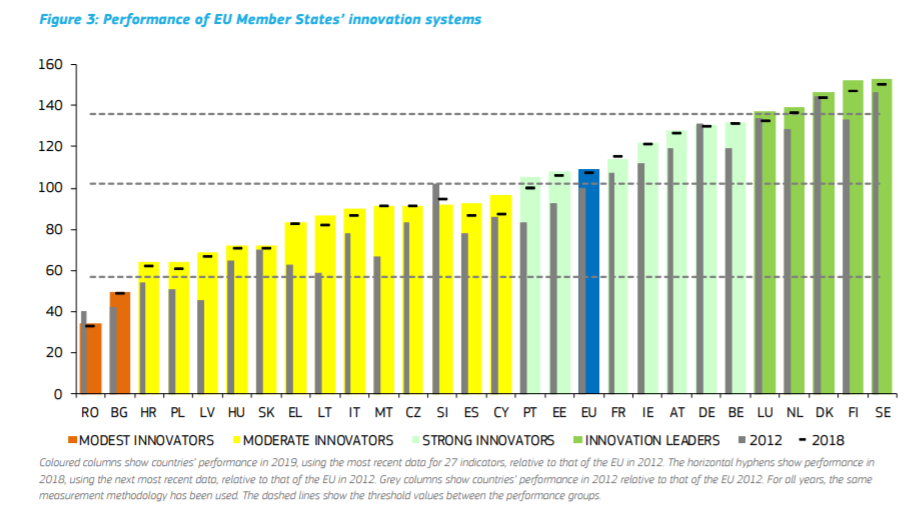
\includegraphics[width=1.\textwidth]{InnovationScoreboard.png}
			\label{fig:figure1}
		\end{figure}
	\end{frame}
	
	\subsection{Innovation Scoreboard - Modest Innovators Group}
	
	\begin{frame}{Table 15 - Model 2 - Modest Innovators}
		\input{MeanTable15_2_modest.tex}
	\end{frame}

	\subsection{Innovation Scoreboard - Moderate Innovators Group}

	\begin{frame}{Table 15 - Model 2 - Moderate Innovators}
		\input{MeanTable15_2_moderate.tex}
	\end{frame}

	\subsection{Innovation Scoreboard - Strong Innovators Group}

	\begin{frame}{Table 15 - Model 2 - Strong Innovators}
		\input{MeanTable15_2_strong.tex}
	\end{frame}

	\subsection{Innovation Scoreboard - Leading Innovators Group}

	\begin{frame}{Table 15 - Model 2 - Leading Innovators}
		\input{MeanTable15_2_leader.tex}
	\end{frame}
	
	\subsection{Innovation Scoreboard - Innovators Group Comparison}	

	\begin{frame}{Table 15 - Model 2 - Group Comparison 1}
		\input{MeanTable15_2_classcomparison_1.tex}
	\end{frame}

	\begin{frame}{Table 15 - Model 2 - Group Comparison 2}
		\input{MeanTable15_2_classcomparison_2.tex}
	\end{frame}

	\begin{frame}{Table 15 - Model 2 - Group Comparison 3}
		\input{MeanTable15_2_classcomparison_3.tex}
	\end{frame}


%	


%	\begin{frame}{Slide with two columns}
%		\begin{columns}
%			\column{.5\textwidth}
%			Text goes in first column.
%			
%			\column{.5\textwidth}
%			Text goes in second column
%		\end{columns}
%	\end{frame}
%	
%	\section{Section Two}
	
%	\begin{frame}{Slide with table}
%		\input{tables/table1.tex}
%	\end{frame}
	
%	\begin{frame}{Slide with figure}
%		\begin{figure}[H]
%			\centering
%			\includegraphics[width=.5\textwidth]{figures/figure1.png}
%			\caption{Caption for figure one.}
%			\label{fig:figure1}
%		\end{figure}
%	\end{frame}
	
%	\begin{frame}{Slide with references}
%		This is to reference a figure (Figure \ref{fig:figure1})\\
%		This it to reference a table (Table \ref{tab:table1})\\
%		This is to cite an article \cite{Ahmed2018a}\\
%		This is to add an article to the references without mentioning in the text \nocite{Ahmed2018a}\\
%	\end{frame}
%	\section{References}
%	
%	% Adding the option 'allowframebreaks' allows the contents of the slide to be expanded in more than one slide.
%	\begin{frame}[allowframebreaks]{References}
%		\tiny\bibliography{references}
%		\bibliographystyle{apalike}
%	\end{frame}
	
\end{document}